\documentclass[10pt, landscape]{article}
\usepackage[scaled=0.92]{helvet}
\usepackage{calc}
\usepackage{multicol}
\usepackage{ifthen}
\usepackage[a4paper,margin=3mm,landscape]{geometry}
\usepackage{amsmath,amsthm,amsfonts,amssymb}
\usepackage{color,graphicx,overpic}
\usepackage{hyperref}
\usepackage{newtxtext} 
\usepackage{enumitem}
\usepackage{amssymb}
\usepackage[table]{xcolor}
\usepackage{vwcol}
\usepackage{tikz}
\usetikzlibrary{arrows.meta}
\usetikzlibrary{calc}
\usepackage{mathtools}
\usepackage{nicematrix}
%For pictures / figures
\usepackage{color,graphicx,overpic}
\graphicspath{ {./images/} }
% for relations
\usepackage{cancel}
\usepackage{ mathrsfs }
\graphicspath{ {./images/} }
\setlist{nosep}


\pdfinfo{
  /Title (CS2030s-PE2.pdf)
  /Creator (TeX)
  /Producer (pdfTeX 1.40.0)
  /Author (Seamus)
  /Subject (Example)
  /Keywords (pdflatex, latex,pdftex,tex)}

% Turn off header and footer
\pagestyle{empty}

\newenvironment{tightcenter}{%
  \setlength\topsep{0pt}
  \setlength\parskip{0pt}
  \begin{center}
}{%
  \end{center}
}

% redefine section commands to use less space
\makeatletter
\renewcommand{\section}{\@startsection{section}{1}{0mm}%
                                {-1ex plus -.5ex minus -.2ex}%
                                {0.5ex plus .2ex}%x
                                {\normalfont\large\bfseries}}
\renewcommand{\subsection}{\@startsection{subsection}{2}{0mm}%
                                {-1explus -.5ex minus -.2ex}%
                                {0.5ex plus .2ex}%
                                {\normalfont\normalsize\bfseries}}
\renewcommand{\subsubsection}{\@startsection{subsubsection}{3}{0mm}%
                                {-1ex plus -.5ex minus -.2ex}%
                                {1ex plus .2ex}%
                                {\normalfont\small\bfseries}}%
\renewcommand{\familydefault}{\sfdefault}
\renewcommand\rmdefault{\sfdefault}
% makes nested numbering (e.g. 1.1.1, 1.1.2, etc)
\renewcommand{\labelenumii}{\theenumii}
\renewcommand{\theenumii}{\theenumi.\arabic{enumii}.}
\renewcommand\labelitemii{•}
%  for logical not operator
\renewcommand{\lnot}{\mathord{\sim}}
\renewcommand{\bf}[1]{\textbf{#1}}
\newcommand{\abs}[1]{\vert #1 \vert}
\newcommand{\Mod}[1]{\ \mathrm{mod}\ #1}

\makeatother
\definecolor{myblue}{cmyk}{1,.72,0,.38}
\everymath\expandafter{\the\everymath \color{myblue}}
% Define BibTeX command
\def\BibTeX{{\rm B\kern-.05em{\sc i\kern-.025em b}\kern-.08em
    T\kern-.1667em\lower.7ex\hbox{E}\kern-.125emX}}
\let\iff\leftrightarrow
\let\Iff\Leftrightarrow
\let\then\rightarrow
\let\Then\Rightarrow

% Don't print section numbers
\setcounter{secnumdepth}{0}

\setlength{\parindent}{0pt}
\setlength{\parskip}{0pt plus 0.5ex}
%% this changes all items (enumerate and itemize)
\setlength{\leftmargini}{0.5cm}
\setlength{\leftmarginii}{0.5cm}
\setlist[itemize,1]{leftmargin=2mm,labelindent=1mm,labelsep=1mm}
\setlist[itemize,2]{leftmargin=4mm,labelindent=1mm,labelsep=1mm}

%My Environments
\newtheorem{example}[section]{Example}
% -----------------------------------------------------------------------

\begin{document}
\raggedright
\footnotesize
\begin{multicols}{4}


% multicol parameters
% These lengths are set only within the two main columns
\setlength{\columnseprule}{0.25pt}
\setlength{\premulticols}{1pt}
\setlength{\postmulticols}{1pt}
\setlength{\multicolsep}{1pt}
\setlength{\columnsep}{2pt}

\begin{center}
    \fbox{%
        \parbox{0.8\linewidth}{\centering \textcolor{black}{
            {\Large\textbf{CS2030S PE2}}
            \\ \normalsize{AY24/25 sem 2}}
            \\ {\footnotesize \textcolor{myblue}{github.com/mendax1234}} 
        }%
    }
\end{center}
\section{Functional Interface}
\begin{enumerate}
    \item (\texttt{BooleanCondition<T>}):
    \begin{itemize}
        \item \textbf{Lambda example}: \texttt{BooleanCondition<Integer> isPositive = x -> x > 0;}
        \item \textbf{Java equivalent}: \texttt{Predicate<T>}.
    \end{itemize}
    \item (\texttt{Producer<T>}): 
    \begin{itemize}
        \item \textbf{Lambda example}: \texttt{Producer<Double> randomValue = () -> Math.random();}
        \item \textbf{Java equivalent}: \texttt{Supplier<T>}.
    \end{itemize}
    \item (\texttt{Consumer<T>}):
    \begin{itemize}
        \item \textbf{Lambda example}: \texttt{Consumer<String> printUpperCase = s -> System.out.println(s.toUpperCase());}
        \item \textbf{Java equivalent}: \texttt{Consumer<T>}
    \end{itemize}
    \item (\texttt{Transformer<U, T>}): Tranform a value of type \texttt{U} into a value of type \texttt{T}.
    \begin{itemize}
        \item \textbf{Lambda example}: \texttt{Transfomer<String, Integer> stringLength = s -> s.length();}
        \item \textbf{Java equivalent}: \texttt{Function<U,T>}
    \end{itemize}
    \item (\texttt{Combiner<S, T, R>}): Combine two values of type \texttt{S, T} into a value of type \texttt{S}.
    \begin{itemize}
        \item \textbf{Lambda example}: \texttt{Combiner<Integer, Integer, Integer> multiply = (a, b) -> a * b;}
        \item \textbf{Java equivalent}: \texttt{BiFunction<S, T, R>}.
    \end{itemize}
    \item \textbf{Functional Interface Example} \\
    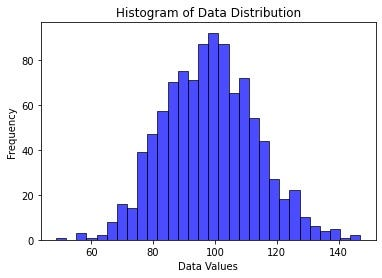
\includegraphics[width=0.8\linewidth]{PE/PE2/images/7.png}
\end{enumerate}

\section{List}
\begin{enumerate}
    \item \textbf{Create an empty List}: 
    \begin{itemize}
        \item \textbf{Create an empty immutable list}: \texttt{List<T> l = List.of();}
        \item \textbf{Create an empty mutable list}: \texttt{List<T> l = new ArrayList<>();}
    \end{itemize}
    \item \textbf{Copy from a List to another}: This is usually used in the \textbf{constructor}, use \texttt{this.fruits = new ArrayList<>(fruits);}, where \texttt{this.fruits} is of type \texttt{List<T>} and \texttt{fruits} is of type \texttt{List<? extends T>} to avoid the type problems. And \texttt{import java.util.ArrayList;}
    \item \textbf{List to stream}: use \texttt{list.stream()}
    \item \textbf{Stream to list}: use \texttt{stream.toList()}
    \item \textbf{isEmpty}: This function can be used to filter out the empty list from the stream. \\
    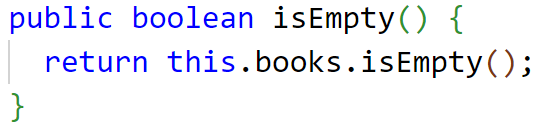
\includegraphics[width=0.8\linewidth]{PE/PE2/images/8.png} \\
    \texttt{filter()} here will keep the elements that are \textbf{not empty}!
    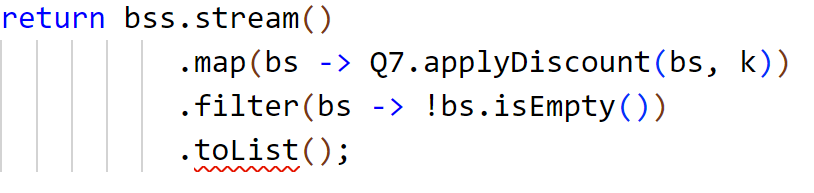
\includegraphics[width=1\linewidth]{PE/PE2/images/9.png}
\end{enumerate}

\section{Maybe}
\begin{enumerate}
    \item \texttt{Maybe.some} always represents a \textbf{valid} value inside the wrapper. \texttt{Maybe.None} always represents \textbf{not found or value DNE}.
    \item \textbf{map}: if the target is \texttt{Maybe.some}, \texttt{map} will always add a \texttt{Maybe.some} wrapper! (Not calling \texttt{Maybe.of}!) \textbf{Can think of map() as a method that will return a value}
    \item \textbf{Use Maybe to rewrite if-else branch}:
    \begin{itemize}
        \item \textbf{Write conditions}: This is usually done by constructing a \texttt{Maybe} and using \texttt{filter}
        \item \textbf{Invoke the method in if-branch}: this can be done by using \texttt{flatMap}/\texttt{map}
        \begin{itemize}
            \item \textbf{To pass several parameters}: Chain \texttt{flatMap()} and \texttt{map()}, the result after this step is still a \texttt{Maybe}.
            \item \textbf{Change a different variable to use}: This can be done using \textbf{flatMap()/map()} also!
            \item \textbf{ifPresent}: this usually after the previous step, if need further operation on the result, use invoke the method using \textbf{ifPresent}. (\textbf{Think it as a function that returns void})
        \end{itemize}
        \item \textbf{Inovke the method in else-branch}: this can be done using \texttt{orElse()}/\texttt{orElseGet()}
        \begin{itemize}
            \item These two methods are usually used to get the value from previous \textbf{Maybe} or produce a new value.
        \end{itemize}
    \end{itemize}
    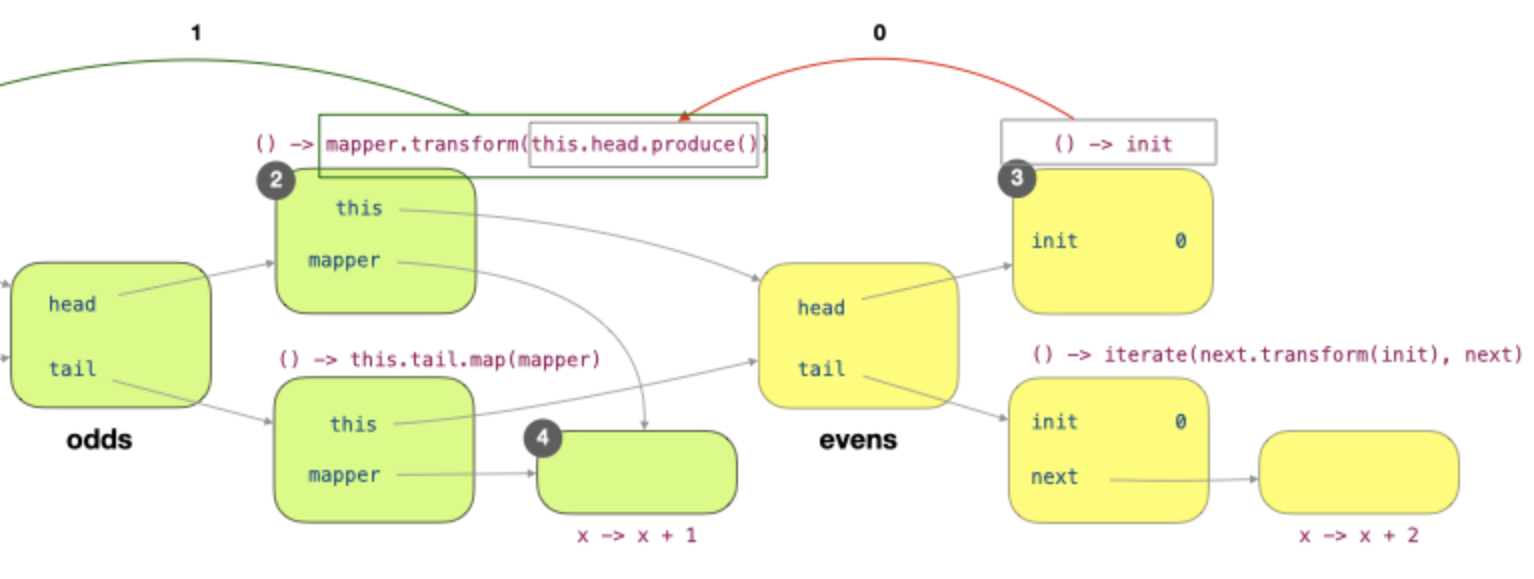
\includegraphics[width=1\linewidth]{PE/PE2/images/3.png}
    \item \textbf{orElse()/orElseGet() Example}: \\
    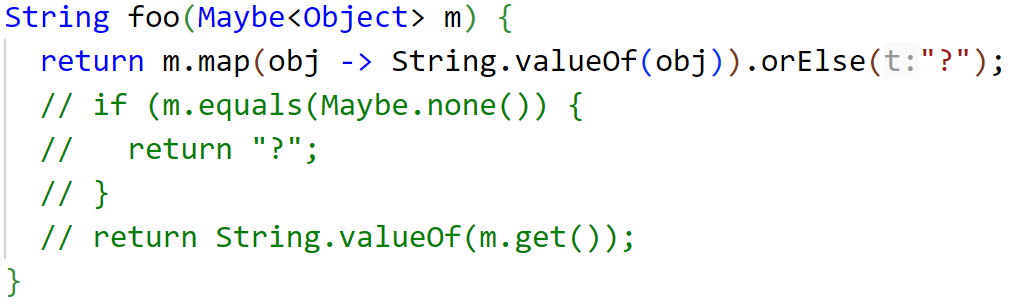
\includegraphics[width=1\linewidth]{PE/PE2/images/15.png}
    \item \textbf{Main Method Descriptor}
    \begin{itemize}
        \item \texttt{filter(BooleanCondition<? super T> c)}: Only keep the value in the \texttt{Maybe} wrapper if it \textbf{pass the test}
        \item \texttt{map(Transformer<? super T, ? extends U> t)}
        \item \texttt{flatMap(Transformer<? super T, ? extends Maybe<? extends U>> t)}
        \item \texttt{orElse(T t)}
        \item \texttt{orElseGet(Producer<? extends T> p)}
        \item \texttt{ifPresent(Consumer<? super T> c)}
        \item \texttt{of(T t)}: if \texttt{t == null}, return \texttt{Maybe.none()}. Else, return \texttt{Maybe.some(t)}.
    \end{itemize}
\end{enumerate}

\section{Lazy}
\begin{enumerate}
    \item \textbf{Basic}: Lazy can store either an \textbf{already existed value} (Wrapped by \texttt{Maybe.some}) or a \textbf{producer which will be used to produce a value}.
    \item \textbf{The memoization thinking} in \texttt{Lazy::get()}, also an example for multiple lines lambda \\
    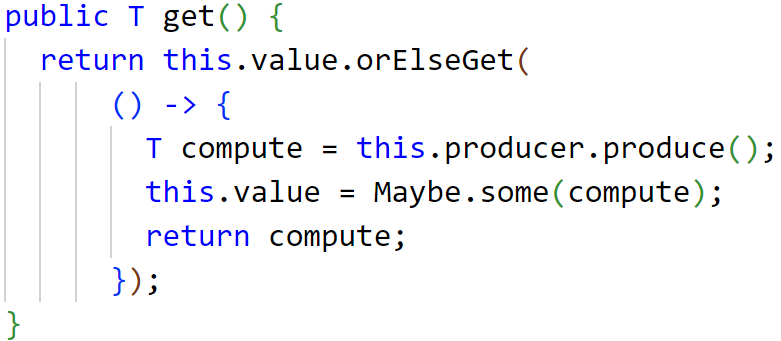
\includegraphics[width=1\linewidth]{PE/PE2/images/16.png}
    \item \textbf{Lazy List Example}: \\
    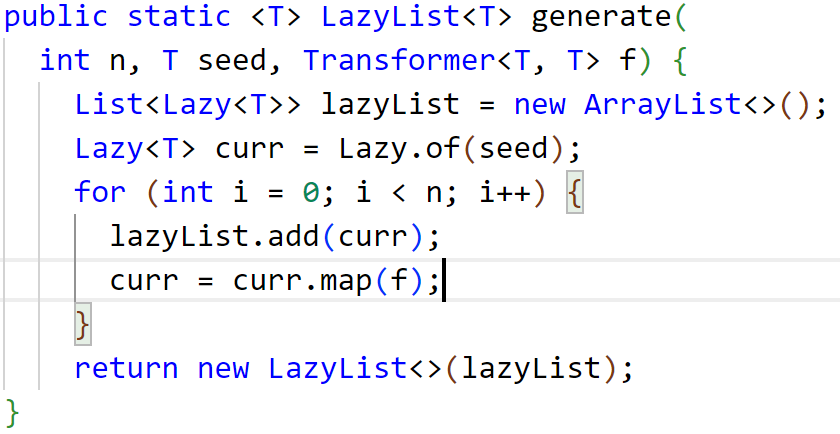
\includegraphics[width=1\linewidth]{PE/PE2/images/13.png}
\end{enumerate}

\section{Infinite List}
\begin{enumerate}
    \item \textbf{Traverse through the infinite list}: \\
    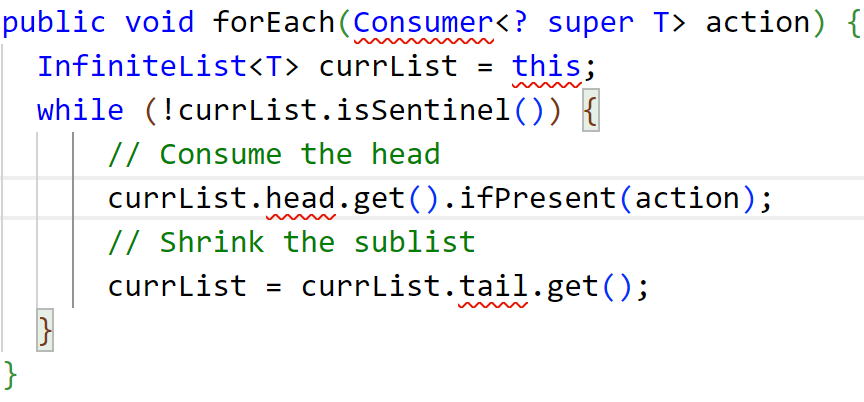
\includegraphics[width=1\linewidth]{PE/PE2/images/14.png}
\end{enumerate}

\section{Stream}
\begin{enumerate}
    \item When using the \textbf{intermediate operation} on stream, use the good practice to write lambda as \texttt{each element -> what operation}. e.g. \texttt{fruits.stream().map(fruit -> String.format("- \%s", fruit));}
    \item \textbf{reduce()}: It's workflow is like that \textbf{result = identity} $\rightarrow$ \textbf{for each element in the stream; result = accumulator.apply(result, element); return result}
    \begin{itemize}
        \item \texttt{reduce(identity, accumulator)}: the \texttt{identity} and \texttt{element in the stream} must be of the \textbf{same} type! \\
        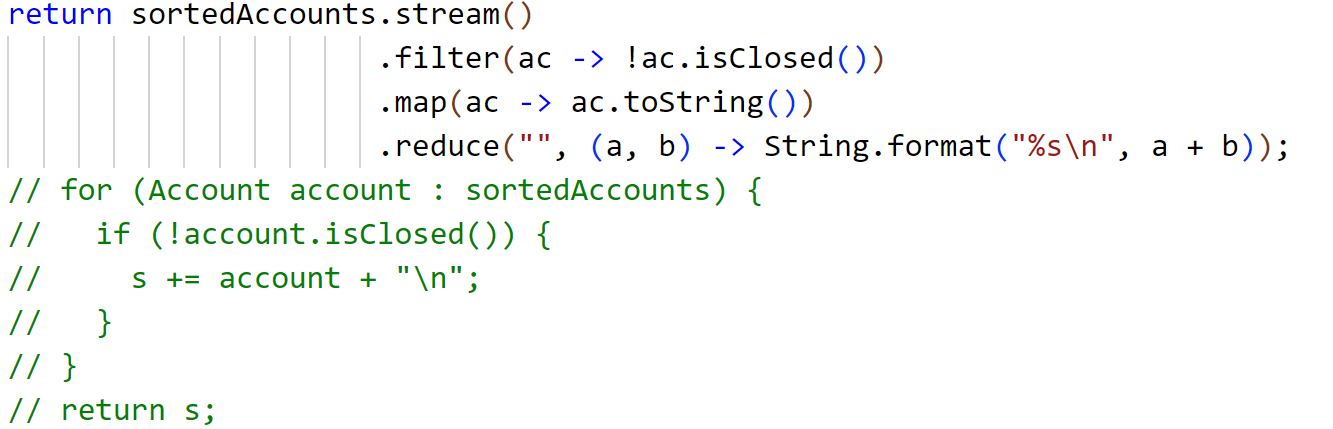
\includegraphics[width=1\linewidth]{PE/PE2/images/1.png}
        \item \texttt{reduce(identity, accumulator, combiner)}: the \textbf{identity} \textbf{may not be the same type} as the \textbf{element in the stream} 
        \begin{itemize}
            \item \textbf{Combiner} is \texttt{(a,b) -> a + b}, this is usually used for the summation of the stream elements.
            \item \textbf{Combiner} is \texttt{(a,b) -> a * b}, this is usually used for the product of the stream elements.
            \item The other Combiner like \texttt{(a,b) -> a - b} and \texttt{(a,b) -> a / b} are \textbf{not safe}! Don't use!
        \end{itemize}
        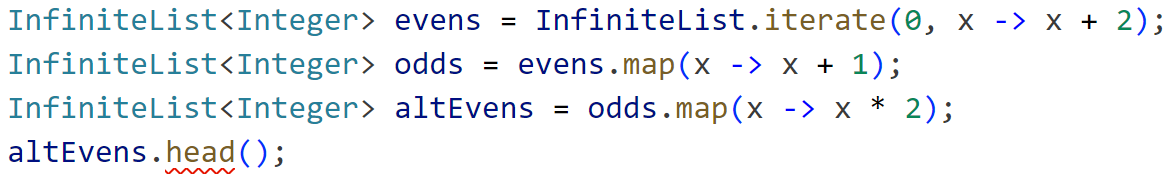
\includegraphics[width=1\linewidth]{PE/PE2/images/2.png}
        \item \textbf{Explicitly cast the return type}: This can be done by changing the type of \textbf{identity} in \texttt{reduce} \\
        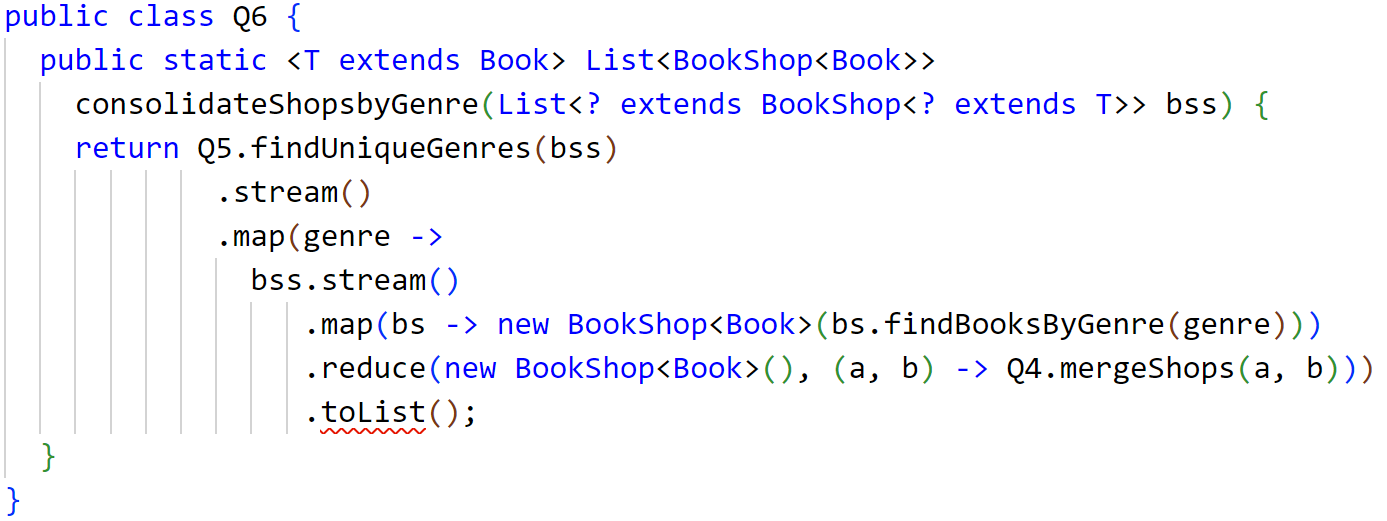
\includegraphics[width=1\linewidth]{PE/PE2/images/12.png}
    \end{itemize}
    \item \textbf{map()}: transforms \textbf{each element} in the stream by \textbf{applying a function (transformer)} to it, producing a new stream of the transformed elements with a \textbf{one-to-one relationship}. \\
    For example, here the \textbf{name} and the \textbf{cost after reducing} has a \textbf{one-to-one} relationship \\
    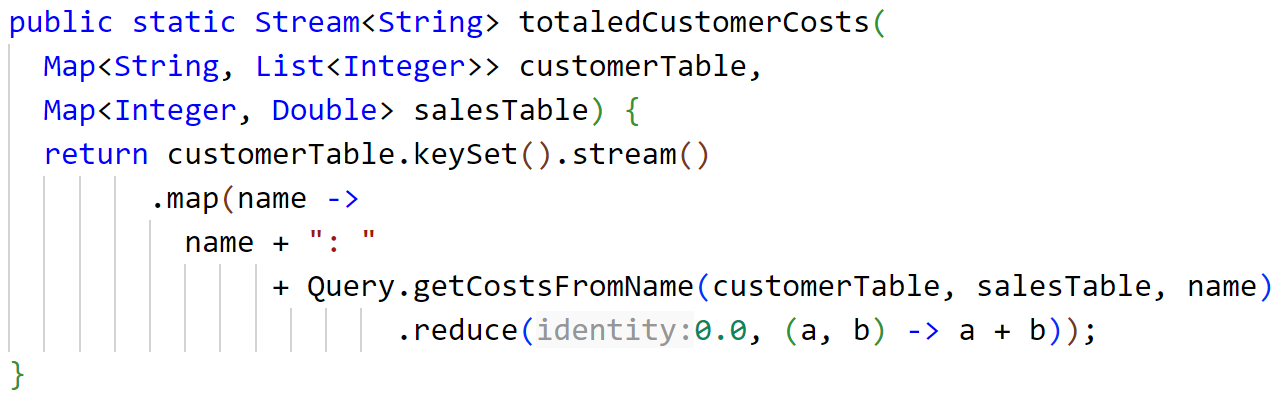
\includegraphics[width=1.0\linewidth]{PE/PE2/images/5.png}
    \item \textbf{flatMap()}: transforms \textbf{each element} into a \textbf{stream} and then \textbf{flattens} all resulting streams into a single stream, useful for working \textbf{with nested collections} or \textbf{when one element should produce multiple output elements}. \\
    For example, here the \textbf{name} and the \textbf{cost} has a \textbf{one-to-multiple} relationship \\
    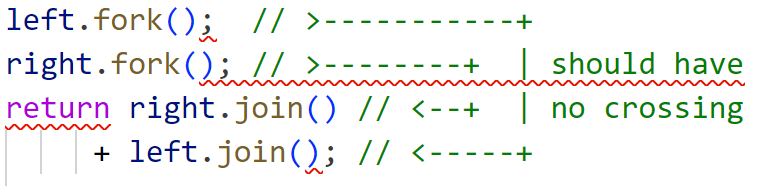
\includegraphics[width=1.0\linewidth]{PE/PE2/images/4.png}
    \item \textbf{filter()}: Creates a new stream that keeps \textbf{only the elements that passed the test} in \texttt{Predicate}.
    \item \textbf{none/any/allMatch()}: a \textbf{boolean} method. It returns \texttt{true} only if \textbf{no/any/all} element in the stream \textbf{passes the predicate test}.
    \item \textbf{sorted()}: elements according to \textbf{natural order} (small to big or ascending order) or a \textbf{provided comparator} \\
    The following provides an example on \texttt{sorted} as well as how to use \texttt{reduce} to find maximum/minimum value in a stream \\
    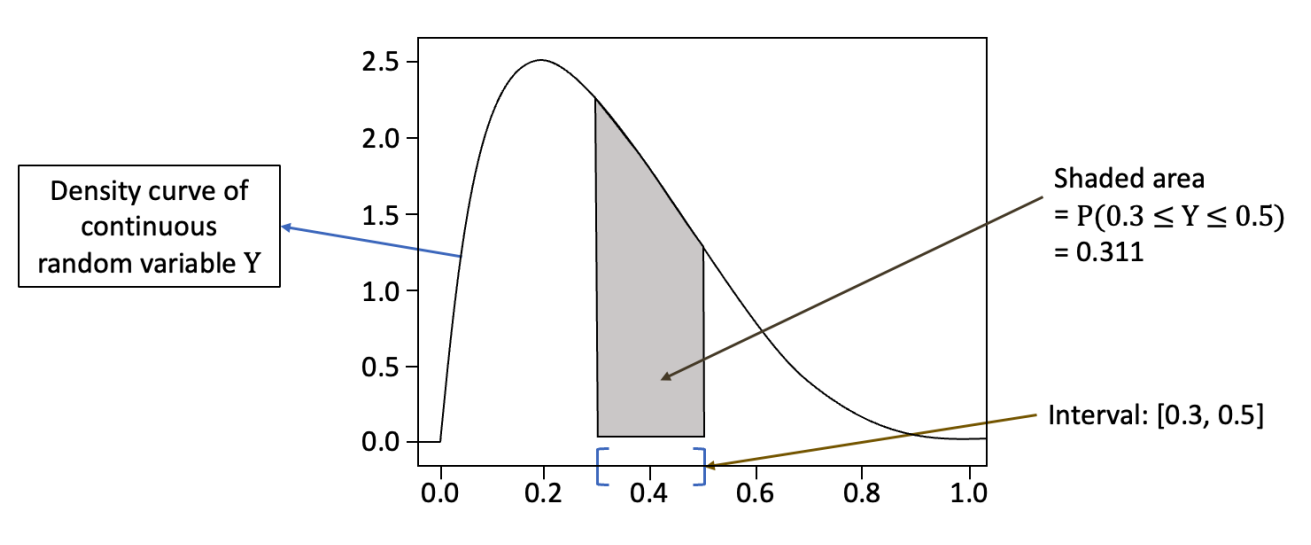
\includegraphics[width=1\linewidth]{PE/PE2/images/10.png}
\end{enumerate}

\section{Monad and Functors}
\begin{enumerate}
    \item \textbf{Monad Laws}:
    \begin{itemize}
        \item \textbf{The left identity law}: \texttt{Monad.of(x).flatMap(x -> f(x))} must be the same as \texttt{f(x)}
        \item \textbf{The right identity law}: \texttt{monad.flatMap(x -> Monad.of(x))} must be the same as \texttt{monad}
        \item \textbf{The associative law}: \texttt{monad.flatMap(x -> f(x)).flatMap(x -> g(x))} must be the same as \texttt{monad.flatMap(x -> f(x).flatMap(y -> g(y)))}
    \end{itemize}
    \item \textbf{Functor Laws}:
    \begin{itemize}
        \item \textbf{Identity Law}: \texttt{functor.map(x -> x)} is the same as \texttt{functor}
        \item \textbf{Composition Law}: \texttt{functor.map(x -> f(x)).map(x -> g(x))} is the same as \texttt{functor.map(x -> g(f(x))}.
    \end{itemize}
\end{enumerate}

\section{Miscs}
\begin{enumerate}
    \item (\textbf{Bounded type parameter}): A type parameter, like \texttt{T} can have a bound! e.g., \texttt{T extends Fruit} means the type parameter \texttt{T} must be a subtype of \texttt{Fruit}.
    \item \textbf{Make your method as flexible as possible!}: Usually, we use \textbf{producer extends} more.
    \item (\textbf{Immutable class}):
    \begin{itemize}
        \item When you are designing a class with a \texttt{List} as its member and you may use stream later, think about making it final to make the class immutable.
        \item For Java \textbf{arrays} and \textbf{String}, just add keyword \texttt{final}.
        \item When return a \textbf{non-primitive} type, \textbf{make a hard copy}! For example, to make a hard copy of \texttt{List}, the first argument is your List object, the second element is the length of your List. \\
        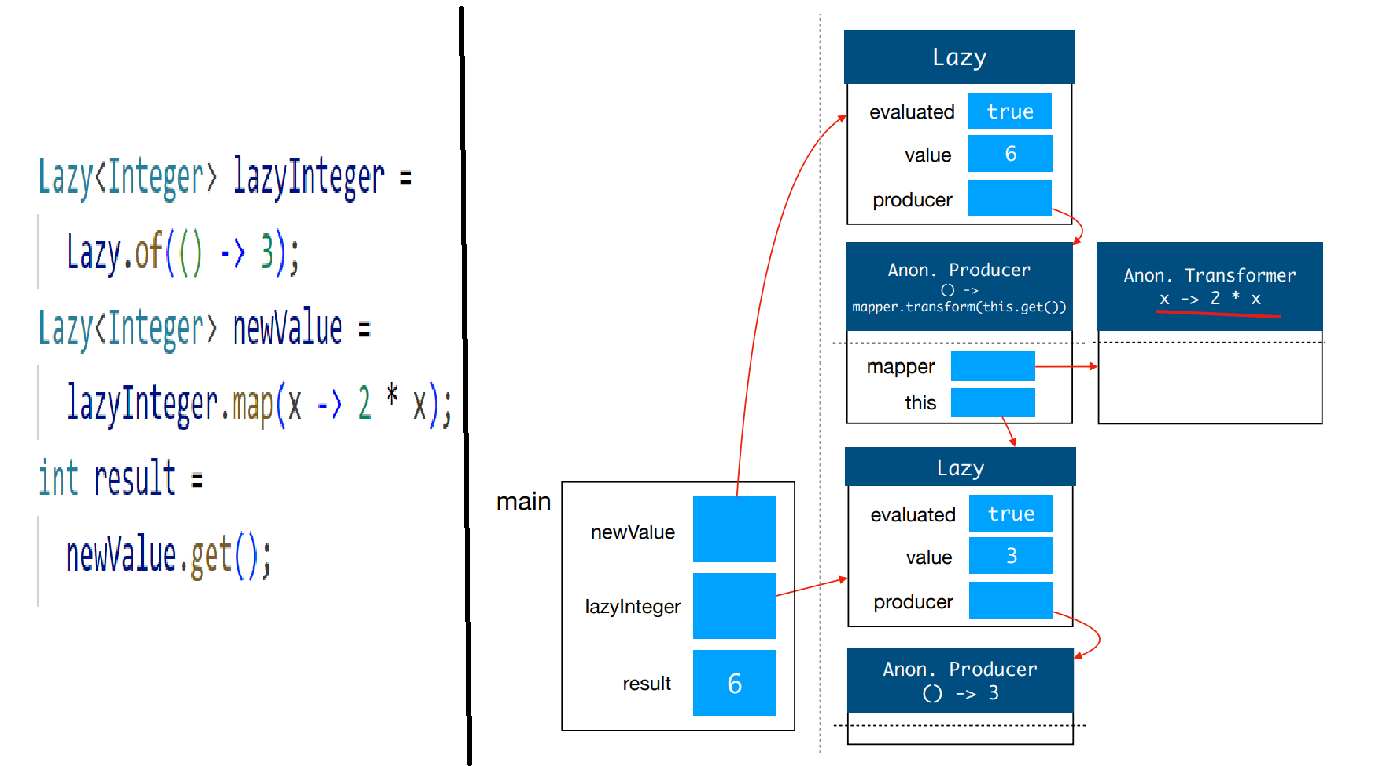
\includegraphics[width=1\linewidth]{PE/PE2/images/6.png}
    \end{itemize}
    \item \textbf{General advice for writing one-liner}
    \begin{itemize}
        \item Start by considering the condition to use (This should be a object of type \texttt{Maybe})
        \item End by using \texttt{orElse()/orElseGet()}.
        \begin{itemize}
            \item Anything between the start and the end is your \textbf{if branch}.
            \item The "placeholder" in your end (in the \texttt{orElse()/orElseGet()}) is the \textbf{else branch}.
        \end{itemize}
    \end{itemize}
    \item \textbf{Print Modifier}: \\
        \[
        \begin{array}{|c|c|}
        \hline
        \textbf{Specifier} & \textbf{Data Type} \\
        \hline
        \%d & \text{Integer (decimal)} \\
        \hline
        \%f & \text{Floating~point (decimal)} \\
        \hline
        \%s & \text{String} \\
        \hline
        \%c & \text{Character} \\
        \hline
        \%b & \text{Boolean} \\
        \hline
        \%\% & \text{Literal \% sign} \\
        \hline
        \end{array}
        \]
        \\
        To print the decimal point, we use \texttt{\%.2f}(2 decimal places)
    \item \textbf{Write a class with one static method}: In case need other methods, can also write like below \\
    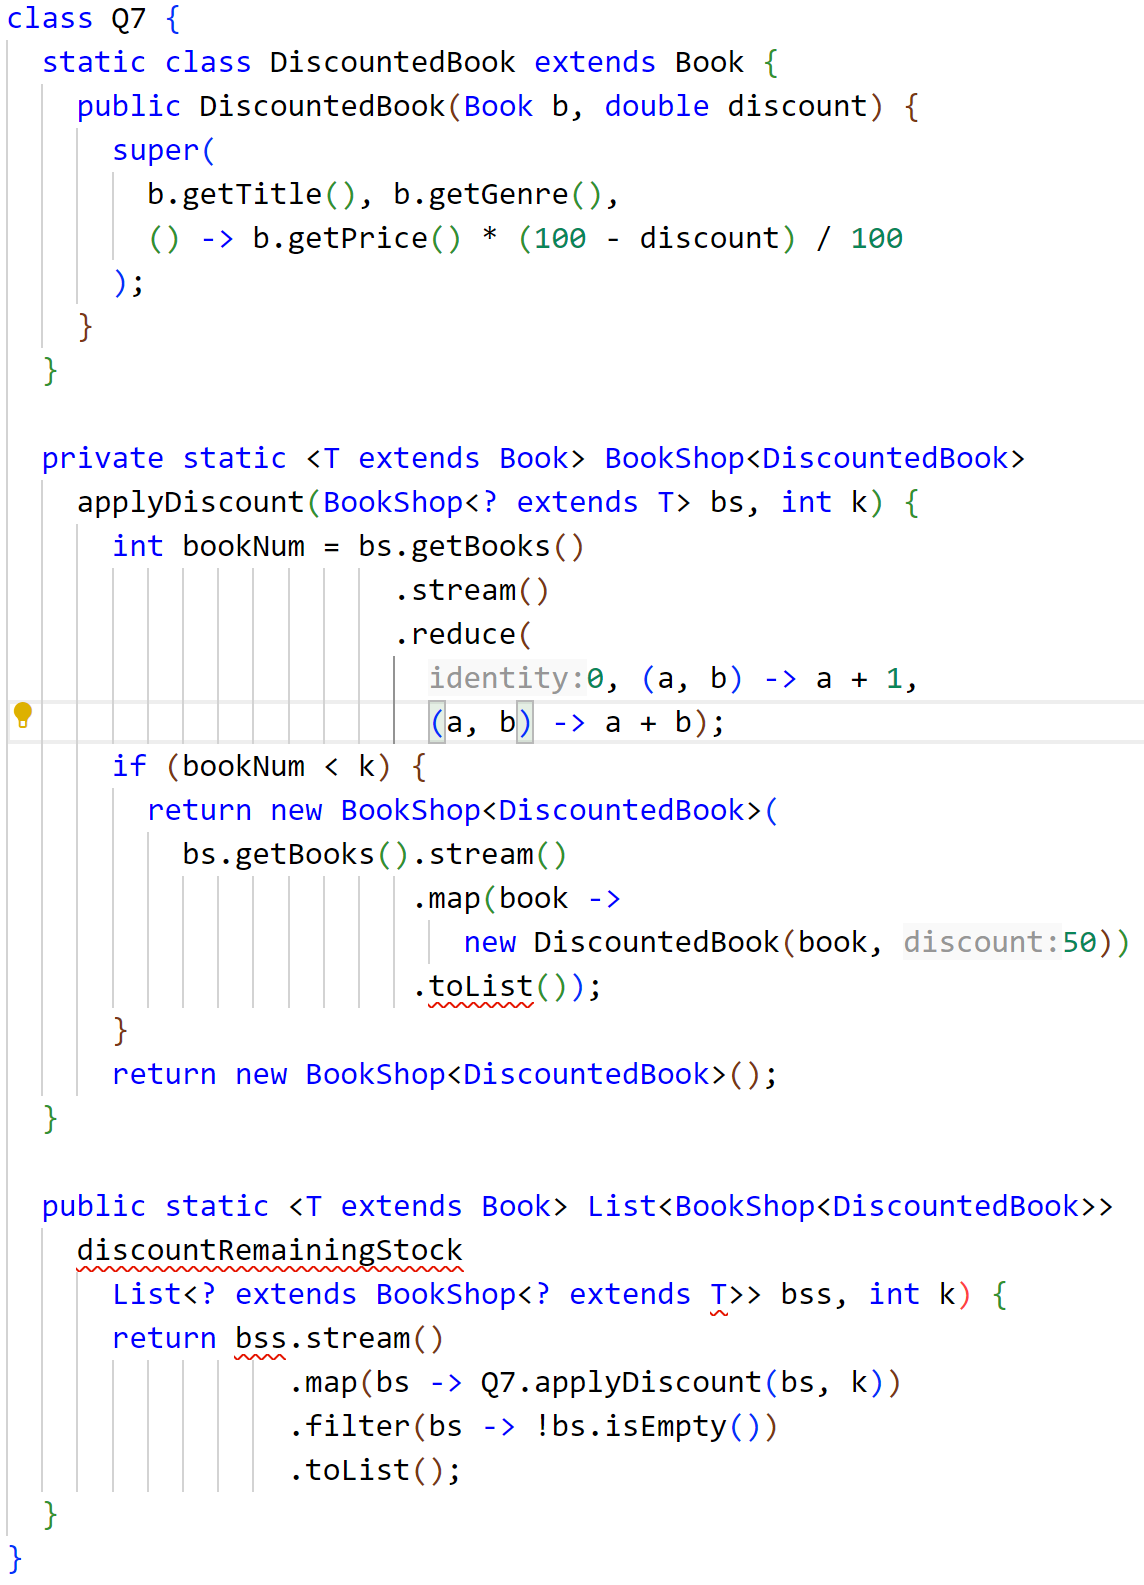
\includegraphics[width=1\linewidth]{PE/PE2/images/11.png}
\end{enumerate}

\end{multicols}

% Dividing Line
\hrulefill \\
\begin{multicols}{3}

\end{multicols}



\end{document}